\section*{\Large{Введение}}
\addcontentsline{toc}{section}{\Large{Введение}}

% Основная мысль: вот пацаны смотрите какой генплан и он типа дофига сложный

Для того чтобы создать любую вещь необходимо сначала её представить.
Если вещь достаточно простая, то весь процесс её создания может спокойно уместиться в голове человека.
Но по мере усложнения устройства той или иной вещи становится невозможно удержать весь контекст в голове,
процесс создания начинает требовать документации.
Если вещь становится совсем сложной, то для её создания требуется уже большое количество специалистов из разных
областей, знакомых с тонкостями той или иной сферы деятельности.

Описанное выше применимо и для сферы строительства.
Любому сложному строительству предшествует этап проектирования.
Результатом этого этапа является генеральный план площадного объекта (пример см. рис\ \ref{pic:introduction__site-plan}).
Именно на его основе проводится оценка, как капитальных, так и эксплуатационных затрат.
За проектирование крупных технологических объектов отвечают проектные институты.
При составлении проекта инженеры-проектировщики опираются на собственный опыт, а также на набор строительных норм
и правил эксплуатации.

\begin{figure}[H]
	\hspace*{-2.5 cm}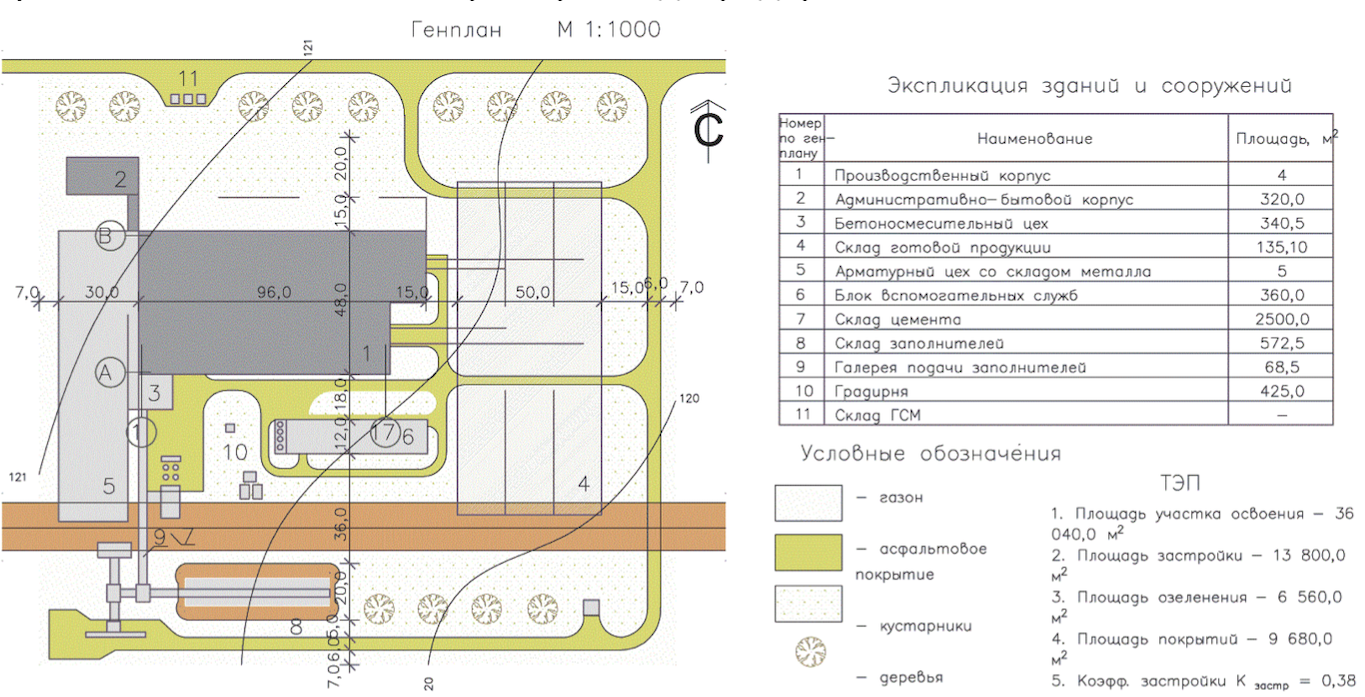
\includegraphics[width=0.5\textwidth]{introduction/pictures/site_plan}
	\caption{Пример генерального плана площадного объекта}
	\label{pic:introduction__site-plan}
\end{figure}
\vskip 5 mm

Инженеры-проектировщики в качестве основного рабочего инструмента используются CAD-системы.
В данных инструментах отсутствует возможность автоматизировать процесс построения конструкции.
По сути, инженер строит решение вручную с нуля, базируясь на требованиях ГОСТ, СНиП, а также своды правил
эксплуатации того или иного сооружения, что является сложным процессом, требующим высокой квалификации специалиста.
